\documentclass[./m2r-pres.tex]{subfile}

%To motivate the key concepts here, we first consider the graph of 6 vertices, with 
%edges joining each point to every other point. This called this the complete graph of order 6, K_6. We can consider colouring 
%the edges either red or blue, shown here.

\begin{frame}
    \frametitle{A motivational example}

    \begin{figure}[h]
        \begin{center}
            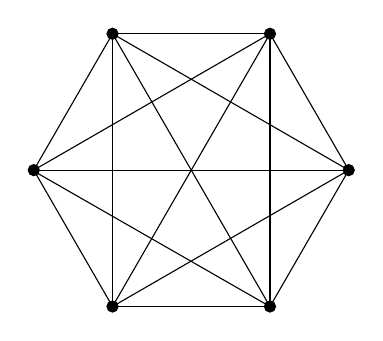
\begin{tikzpicture}
                \draw (0,0) -- (2,0);
                \draw (2,0) -- (3,1.7321);
                \draw (3,1.7321) -- (2,3.4641);
                \draw (2,3.4641) -- (0,3.4641);
                \draw (0,3.4641) -- (-1,1.7321);
                \draw (-1,1.7321) -- (0,0);
                \draw (0,0) -- (2,3.4641);
                \draw (3,1.7321) -- (-1,1.7321);
                \draw (2,0) -- (0,3.4641);
        
                \draw (0,0) -- (3,1.7321);
                \draw (3,1.7321) -- (0,3.4641);
                \draw (0,3.4641) -- (0,0);
                \draw (2,0) -- (2,3.4641);
                \draw (2,3.4641) -- (-1,1.7321);
                \draw (-1,1.72,0) -- (2,0);
        
                \filldraw (0,0) circle (2pt);
                \filldraw (2,0) circle (2pt);
                \filldraw (3,1.7321) circle (2pt);
                \filldraw (2,3.4641) circle (2pt);
                \filldraw (0,3.4641) circle (2pt);
                \filldraw (-1,1.7321) circle (2pt);
            \end{tikzpicture}
        
        \end{center}
        \caption{$K_6$}
  
    \end{figure}
    
\end{frame}

\begin{frame}
    \frametitle{A motivational example}

    \begin{figure}[h]
        \begin{center}
            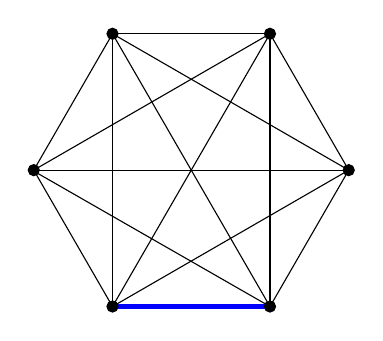
\begin{tikzpicture}
                \draw [blue, line width=2pt] (0,0) -- (2,0);
                \draw (2,0) -- (3,1.7321);
                \draw (3,1.7321) -- (2,3.4641);
                \draw (2,3.4641) -- (0,3.4641);
                \draw (0,3.4641) -- (-1,1.7321);
                \draw (-1,1.7321) -- (0,0);
                \draw (0,0) -- (2,3.4641);
                \draw (3,1.7321) -- (-1,1.7321);
                \draw (2,0) -- (0,3.4641);
        
                \draw (0,0) -- (3,1.7321);
                \draw (3,1.7321) -- (0,3.4641);
                \draw (0,3.4641) -- (0,0);
                \draw (2,0) -- (2,3.4641);
                \draw (2,3.4641) -- (-1,1.7321);
                \draw (-1,1.72,0) -- (2,0);
        
                \filldraw (0,0) circle (2pt);
                \filldraw (2,0) circle (2pt);
                \filldraw (3,1.7321) circle (2pt);
                \filldraw (2,3.4641) circle (2pt);
                \filldraw (0,3.4641) circle (2pt);
                \filldraw (-1,1.7321) circle (2pt);
            \end{tikzpicture}
        
        \end{center}
        \caption{$K_6$}
  
    \end{figure}
    
\end{frame}

\begin{frame}
    \frametitle{A motivational example}

    \begin{figure}[h]
        \begin{center}
            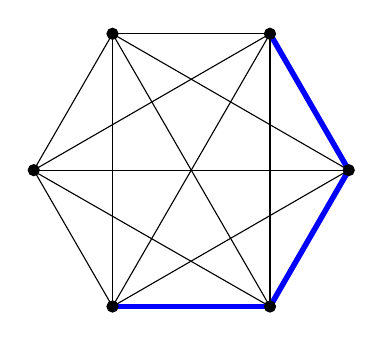
\begin{tikzpicture}
                \draw [blue, line width=2pt] (0,0) -- (2,0);
                \draw [blue, line width=2pt] (2,0) -- (3,1.7321);
                \draw [blue, line width=2pt] (3,1.7321) -- (2,3.4641);
                \draw (2,3.4641) -- (0,3.4641);
                \draw (0,3.4641) -- (-1,1.7321);
                \draw (-1,1.7321) -- (0,0);
                \draw (0,0) -- (2,3.4641);
                \draw (3,1.7321) -- (-1,1.7321);
                \draw (2,0) -- (0,3.4641);
        
                \draw (0,0) -- (3,1.7321);
                \draw (3,1.7321) -- (0,3.4641);
                \draw (0,3.4641) -- (0,0);
                \draw (2,0) -- (2,3.4641);
                \draw (2,3.4641) -- (-1,1.7321);
                \draw (-1,1.72,0) -- (2,0);
        
                \filldraw (0,0) circle (2pt);
                \filldraw (2,0) circle (2pt);
                \filldraw (3,1.7321) circle (2pt);
                \filldraw (2,3.4641) circle (2pt);
                \filldraw (0,3.4641) circle (2pt);
                \filldraw (-1,1.7321) circle (2pt);
            \end{tikzpicture}
        
        \end{center}
        \caption{$K_6$}
  
    \end{figure}
    
\end{frame}

\begin{frame}
    \frametitle{A motivational example}

    \begin{figure}[h]
        \begin{center}
            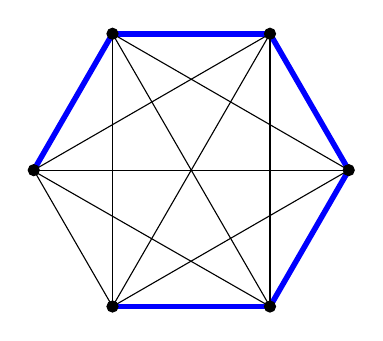
\begin{tikzpicture}
                \draw [blue, line width=2pt] (0,0) -- (2,0);
                \draw [blue, line width=2pt] (2,0) -- (3,1.7321);
                \draw [blue, line width=2pt] (3,1.7321) -- (2,3.4641);
                \draw [blue, line width=2pt] (2,3.4641) -- (0,3.4641);
                \draw [blue, line width=2pt] (0,3.4641) -- (-1,1.7321);
                \draw (-1,1.7321) -- (0,0);
                \draw (0,0) -- (2,3.4641);
                \draw (3,1.7321) -- (-1,1.7321);
                \draw (2,0) -- (0,3.4641);
        
                \draw (0,0) -- (3,1.7321);
                \draw (3,1.7321) -- (0,3.4641);
                \draw (0,3.4641) -- (0,0);
                \draw (2,0) -- (2,3.4641);
                \draw (2,3.4641) -- (-1,1.7321);
                \draw (-1,1.72,0) -- (2,0);
        
                \filldraw (0,0) circle (2pt);
                \filldraw (2,0) circle (2pt);
                \filldraw (3,1.7321) circle (2pt);
                \filldraw (2,3.4641) circle (2pt);
                \filldraw (0,3.4641) circle (2pt);
                \filldraw (-1,1.7321) circle (2pt);
            \end{tikzpicture}
        
        \end{center}
        \caption{$K_6$}
  
    \end{figure}
    
\end{frame}

\begin{frame}
    \frametitle{A motivational example}

    \begin{figure}[h]
        \begin{center}
            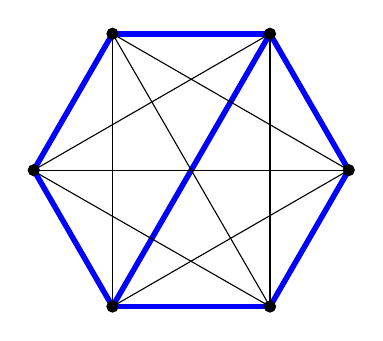
\begin{tikzpicture}
                \draw [blue, line width=2pt] (0,0) -- (2,0);
                \draw [blue, line width=2pt] (2,0) -- (3,1.7321);
                \draw [blue, line width=2pt] (3,1.7321) -- (2,3.4641);
                \draw [blue, line width=2pt] (2,3.4641) -- (0,3.4641);
                \draw [blue, line width=2pt] (0,3.4641) -- (-1,1.7321);
                \draw [blue, line width=2pt] (-1,1.7321) -- (0,0);
                \draw [blue, line width=2pt] (0,0) -- (2,3.4641);
                \draw (3,1.7321) -- (-1,1.7321);
                \draw (2,0) -- (0,3.4641);
        
                \draw (0,0) -- (3,1.7321);
                \draw (3,1.7321) -- (0,3.4641);
                \draw (0,3.4641) -- (0,0);
                \draw (2,0) -- (2,3.4641);
                \draw (2,3.4641) -- (-1,1.7321);
                \draw (-1,1.72,0) -- (2,0);
        
                \filldraw (0,0) circle (2pt);
                \filldraw (2,0) circle (2pt);
                \filldraw (3,1.7321) circle (2pt);
                \filldraw (2,3.4641) circle (2pt);
                \filldraw (0,3.4641) circle (2pt);
                \filldraw (-1,1.7321) circle (2pt);
            \end{tikzpicture}
        
        \end{center}
        \caption{$K_6$}
  
    \end{figure}
    
\end{frame}

\begin{frame}
    \frametitle{A motivational example}

    \begin{figure}[h]
        \begin{center}
            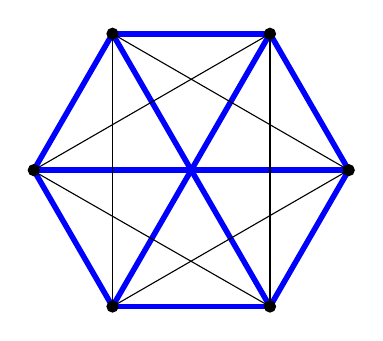
\begin{tikzpicture}
                \draw [blue, line width=2pt] (0,0) -- (2,0);
                \draw [blue, line width=2pt] (2,0) -- (3,1.7321);
                \draw [blue, line width=2pt] (3,1.7321) -- (2,3.4641);
                \draw [blue, line width=2pt] (2,3.4641) -- (0,3.4641);
                \draw [blue, line width=2pt] (0,3.4641) -- (-1,1.7321);
                \draw [blue, line width=2pt] (-1,1.7321) -- (0,0);
                \draw [blue, line width=2pt] (0,0) -- (2,3.4641);
                \draw [blue, line width=2pt] (3,1.7321) -- (-1,1.7321);
                \draw [blue, line width=2pt] (2,0) -- (0,3.4641);
        
                \draw (0,0) -- (3,1.7321);
                \draw (3,1.7321) -- (0,3.4641);
                \draw (0,3.4641) -- (0,0);
                \draw (2,0) -- (2,3.4641);
                \draw (2,3.4641) -- (-1,1.7321);
                \draw (-1,1.72,0) -- (2,0);
        
                \filldraw (0,0) circle (2pt);
                \filldraw (2,0) circle (2pt);
                \filldraw (3,1.7321) circle (2pt);
                \filldraw (2,3.4641) circle (2pt);
                \filldraw (0,3.4641) circle (2pt);
                \filldraw (-1,1.7321) circle (2pt);
            \end{tikzpicture}
        
        \end{center}
        \caption{$K_6$}
  
    \end{figure}
    
\end{frame}

\begin{frame}
    \frametitle{A motivational example}

    \begin{figure}[h]
        \begin{center}
            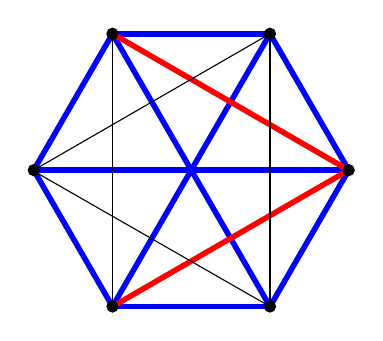
\begin{tikzpicture}
                \draw [blue, line width=2pt] (0,0) -- (2,0);
                \draw [blue, line width=2pt] (2,0) -- (3,1.7321);
                \draw [blue, line width=2pt] (3,1.7321) -- (2,3.4641);
                \draw [blue, line width=2pt] (2,3.4641) -- (0,3.4641);
                \draw [blue, line width=2pt] (0,3.4641) -- (-1,1.7321);
                \draw [blue, line width=2pt] (-1,1.7321) -- (0,0);
                \draw [blue, line width=2pt] (0,0) -- (2,3.4641);
                \draw [blue, line width=2pt] (3,1.7321) -- (-1,1.7321);
                \draw [blue, line width=2pt] (2,0) -- (0,3.4641);
        
                \draw [red, line width=2pt] (0,0) -- (3,1.7321);
                \draw [red, line width=2pt] (3,1.7321) -- (0,3.4641);
                \draw (0,3.4641) -- (0,0);
                \draw (2,0) -- (2,3.4641);
                \draw (2,3.4641) -- (-1,1.7321);
                \draw (-1,1.72,0) -- (2,0);
        
                \filldraw (0,0) circle (2pt);
                \filldraw (2,0) circle (2pt);
                \filldraw (3,1.7321) circle (2pt);
                \filldraw (2,3.4641) circle (2pt);
                \filldraw (0,3.4641) circle (2pt);
                \filldraw (-1,1.7321) circle (2pt);
            \end{tikzpicture}
        
        \end{center}
        \caption{$K_6$}
  
    \end{figure}
    
\end{frame}

\begin{frame}
    \frametitle{A motivational example}

    \begin{figure}[h]
        \begin{center}
            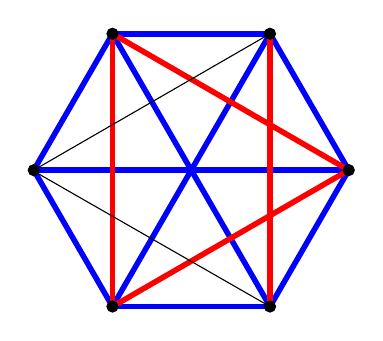
\begin{tikzpicture}
                \draw [blue, line width=2pt] (0,0) -- (2,0);
                \draw [blue, line width=2pt] (2,0) -- (3,1.7321);
                \draw [blue, line width=2pt] (3,1.7321) -- (2,3.4641);
                \draw [blue, line width=2pt] (2,3.4641) -- (0,3.4641);
                \draw [blue, line width=2pt] (0,3.4641) -- (-1,1.7321);
                \draw [blue, line width=2pt] (-1,1.7321) -- (0,0);
                \draw [blue, line width=2pt] (0,0) -- (2,3.4641);
                \draw [blue, line width=2pt] (3,1.7321) -- (-1,1.7321);
                \draw [blue, line width=2pt] (2,0) -- (0,3.4641);
        
                \draw [red, line width=2pt] (0,0) -- (3,1.7321);
                \draw [red, line width=2pt] (3,1.7321) -- (0,3.4641);
                \draw [red, line width=2pt] (0,3.4641) -- (0,0);
                \draw [red, line width=2pt] (2,0) -- (2,3.4641);
                \draw (2,3.4641) -- (-1,1.7321);
                \draw (-1,1.72,0) -- (2,0);
        
                \filldraw (0,0) circle (2pt);
                \filldraw (2,0) circle (2pt);
                \filldraw (3,1.7321) circle (2pt);
                \filldraw (2,3.4641) circle (2pt);
                \filldraw (0,3.4641) circle (2pt);
                \filldraw (-1,1.7321) circle (2pt);
            \end{tikzpicture}
        
        \end{center}
        \caption{$K_6$}
    \end{figure}
    
\end{frame} 

\begin{frame}
    \frametitle{A motivational example}

    \begin{figure}[h]
        \begin{center}
            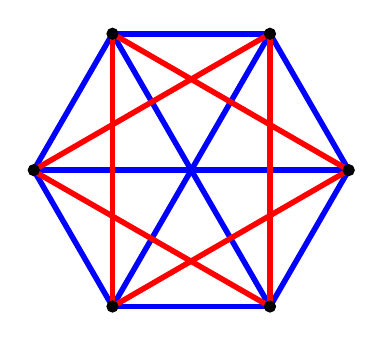
\begin{tikzpicture}
                \draw [blue, line width=2pt] (0,0) -- (2,0);
                \draw [blue, line width=2pt] (2,0) -- (3,1.7321);
                \draw [blue, line width=2pt] (3,1.7321) -- (2,3.4641);
                \draw [blue, line width=2pt] (2,3.4641) -- (0,3.4641);
                \draw [blue, line width=2pt] (0,3.4641) -- (-1,1.7321);
                \draw [blue, line width=2pt] (-1,1.7321) -- (0,0);
                \draw [blue, line width=2pt] (0,0) -- (2,3.4641);
                \draw [blue, line width=2pt] (3,1.7321) -- (-1,1.7321);
                \draw [blue, line width=2pt] (2,0) -- (0,3.4641);
        
                \draw [red, line width=2pt] (0,0) -- (3,1.7321);
                \draw [red, line width=2pt] (3,1.7321) -- (0,3.4641);
                \draw [red, line width=2pt] (0,3.4641) -- (0,0);
                \draw [red, line width=2pt] (2,0) -- (2,3.4641);
                \draw [red, line width=2pt] (2,3.4641) -- (-1,1.7321);
                \draw [red, line width=2pt] (-1,1.72,0) -- (2,0);
        
                \filldraw (0,0) circle (2pt);
                \filldraw (2,0) circle (2pt);
                \filldraw (3,1.7321) circle (2pt);
                \filldraw (2,3.4641) circle (2pt);
                \filldraw (0,3.4641) circle (2pt);
                \filldraw (-1,1.7321) circle (2pt);
            \end{tikzpicture}
        
        \end{center}  
        \caption{2 red triangles within $K_6$}     
    \end{figure}
    
\end{frame} 

%When we've coloured all the edges, we find that we get 2 red triangles. In fact, 
%no matter how we colour the edges, Ramsey's theorem 
%states that we will always get red triangles or blue triangles.

%Notice that adding a any number of vertices does not affect the existence of the monochromatic 
%triangles.
%However, if we take a vertex away from the graph and consider the edge colouring 
%shown here, we can't find any red or blue triangles.

\begin{frame}
    \frametitle{A pathological example}

    \begin{figure}[h]
        \begin{center}
            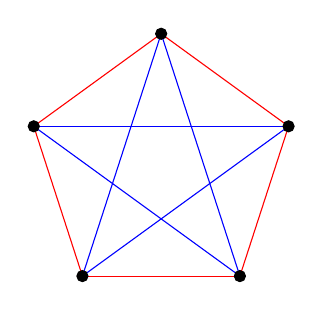
\begin{tikzpicture}
                \draw [red] (0,0) -- (2,0);
                \draw [red] (2,0) -- (2.618,1.9022);
                \draw [red] (2.618,1.9022) -- (1,3.0776);
                \draw [red] (1,3.0776) -- (-0.618,1.9022);
                \draw [red] (-0.618,1.9022) -- (0,0);

                \draw [blue] (0,0) -- (2.618,1.9022);
                \draw [blue] (0,0) -- (1,3.0776);
                \draw [blue] (2,0) -- (1,3.0776);
                \draw [blue] (2,0) -- (-0.618,1.9022);
                \draw [blue] (2.618,1.9022) -- (-0.618,1.9022);
        
                \filldraw (0,0) circle (2pt);
                \filldraw (2,0) circle (2pt);
                \filldraw (2.618,1.9022) circle (2pt);
                \filldraw (1,3.0776) circle (2pt);
                \filldraw (-0.618,1.9022) circle (2pt);
            \end{tikzpicture}
        
        \end{center}
        
        \caption{A particular 2-colouring}
    \end{figure}

\end{frame}

%So we have found that 6 is minimum 
%number of vertices of a graph needed in to ensure the existence of monochromatic triangles. This motivates 
%the definition of Ramsey numbers.
%
%First some definitions:

% \begin{frame}
%     \frametitle{Definitions}

%     \begin{definition}[Colouring]
%     An \textit{$r$-colouring} of a graph $G=(V,E)$, is a partition of the edges $E$ 
%     into $r$ disjoint classes, which is induced by the map 
%     $$\chi: E \to \{1,2,\ldots,r\},\text{     for } r\in\Z^+.$$
%     We say a subset of edges $E'\subset E$ is \textit{monochromatic} if the restriction 
%     $\chi|_{E'}$ is the constant map.
%     \end{definition}
% \end{frame}

\begin{frame}
    \frametitle{Definitions}

    \begin{itemize}
    \item[]<1-> 
    \begin{definition}[Colouring]
        An \textit{$r$-colouring} of a graph $G=(V,E)$, is a partition of the edges $E$ 
        into $r$ disjoint classes, which is induced by the map 
        $$\chi: E \to \{1,2,\ldots,r\},\text{     for } r\in\Z^+.$$
        We say a subset of edges $E'\subset E$ is \textit{monochromatic} if the restriction 
        $\chi|_{E'}$ is the constant map.
    \end{definition}
    \item[]<2->
    \begin{definition}[Complete graph]
    We say a graph is \textit{complete} if every two vertices are joined by an edge. 
    We denote the complete graph of order $n$ by $K_n$.
    \end{definition}
    \end{itemize}
\end{frame}

% \begin{frame}
%     \frametitle{Ramsey's Theorem}

%     \begin{definition}[Ramsey number]

%         For $s,t\in\Z^+$, we define the \textit{Ramsey number} of $s$ and $t$, $R(s,t)$, 
%         to be the least positive integer such that any 2-colouring of $K_n$ contains
%         as a subgraph a monochromatic $K_s$ or a monochromatic $K_t$, whenever 
%         $n\geq R(s,t)$.\\

%         So $R(3,3)=6$. 
%     \end{definition}

% \end{frame}

\begin{frame}
    \frametitle{Ramsey's Theorem}

    \begin{itemize}
    \item[]<1-> 
    \begin{definition}[Ramsey number]

        For $s,t\in\Z^+$, we define the \textit{Ramsey number} of $s$ and $t$, $R(s,t)$, 
        to be the least positive integer such that any 2-colouring of $K_n$ contains
        as a subgraph a monochromatic $K_s$ or a monochromatic $K_t$, whenever 
        $n\geq R(s,t)$.\\

        So $R(3,3)=6$. 
    \end{definition}
    \item[]<2->
    \begin{prop}
    $R(s,t)$ is a well-defined function for all $s,t\in\Z^+.$
    %i.e. for any red-blue colouring of a complete graph of order at least 
    %R(s,t), we can always find a monochromatic complete subgraph of order s or t
    \end{prop}
    \end{itemize}
\end{frame}

%In fact, we can colour the edges of a graph with any finite number of colours, 
%and Ramsey's theorem still holds.

\begin{frame}
    \frametitle{Generalisation to $r$ colours}
    \begin{definition}
    For $s_1,\ldots,s_r\in\Z^+$, we define $R(s_1,\ldots,s_r)$ 
    to be the least positive integer such that any $r$-colouring of $K_n$ contains 
    a complete monochromatic subgraph $K_{s_i}$ whenever 
    $n\geq R(s_1,\ldots,s_r)$, for some $i\in\{1,\ldots,r\}$.\\
    %So here the R(s_1 to s_r) is the Ramsey number for r colours

    For example, $R(3,3,3)=17$.
    %17 is the minimum order of a complete graph such that nomatter how we colour the 
    %edges with 3 colours, we always get a monochromatic triangle
    \end{definition}
\end{frame}

\begin{frame}
    \frametitle{Generalisation to $r$ colours}
    \begin{itemize}
    \item[]<1-> 
    \begin{definition}
    For $s_1,\ldots,s_r\in\Z^+$, we define $R(s_1,\ldots,s_r)$ 
    to be the least positive integer such that any r-colouring of $K_n$ contains 
    a complete monochromatic subgraph $K_{s_i}$ whenever 
    $n\geq R(s_1,\ldots,s_r)$, for some $i\in\{1,\ldots,r\}$.\\

    For example, $R(3,3,3)=17$.
    \end{definition}
    \item[]<2->
    \begin{theorem}
        $R(s_1,\ldots,s_r)$ is a well-defined function for all $s_1,\ldots,s_r\in\Z^+.$
        %i.e. for any set of positive integers s_i and any r colouring of a complete 
        %graph of order at least R(s_1,\ldots,s_r), we can always find a monochromatic
        %complete subgraph of order s_i, for some i.
    \end{theorem}
    \end{itemize}
\end{frame}

%The statement of Ramsey's original theorem 
%concerns partitioning a countably infinite set into a finite number of 
%disjoint subsets

% \begin{frame}
%     \frametitle{Infinite Graphs}
%     \begin{definition}[Infinite complete graph]

%         Let $\Gamma$ be a countably infinite set. We define the 
%         \textit{infinite complete graph}, $K_\infty$, as the ordered pair 
%         $K_\infty:=(\Gamma,\Gamma^{(2)})$.\\

%         Here, $\Gamma^{(2)}$ is the set of all the edges joining each vertex in 
%         $\Gamma$ to every other vertex.
    
%     \end{definition}
% \end{frame}

\begin{frame}
    \frametitle{Infinite Graphs}

    \begin{itemize}
    \item[]<1-> 
    \begin{definition}[Infinite complete graph]

        Let $\Gamma$ be a countably infinite set. We define the 
        \textit{infinite complete graph}, $K_\infty$, as the ordered pair 
        $K_\infty:=(\Gamma,\Gamma^{(2)})$.\\

        Here, $\Gamma^{(2)}$ is the set of all the edges joining each vertex in 
        $\Gamma$ to every other vertex.
    
    \end{definition}
    \item[]<2->
    \begin{theorem}[Ramsey]
        For any r-colouring of $K_\infty$, say
        $\chi :\Gamma^{(2)}\to\{1,\ldots,r\}$, there exists 
        within it a countably infinite monochromatic complete subgraph. In other words, there 
        exists $X \subset K_\infty$ such that $X$ is countably infinite, and $\chi|_{X^{(2)}}$ is the
        constant function.
    \end{theorem}
    %For any r colouring of the infinite graph, there exists a countably infinite 
    %monochromatic complete subgraph

\end{frame}

%An interesting corollary of this result is the following key theorem from 
%analysis:

% \begin{frame}
%     \frametitle{Bolzano-Weierstrass Theorem}
%     \begin{theorem}[Bolzano-Weierstrass]
%         Let $(x_i)_{i\in \Z_+}$ be a bounded sequence of real numbers. Then it has
%         a convergent subsequence.
%     \end{theorem}
% \end{frame}

\begin{frame}
    \frametitle{Bolzano-Weierstrass Theorem}

    \begin{itemize}
    \item[]<1-> 
      \begin{theorem}[Bolzano-Weierstrass]
        Let $(x_i)_{i\in \Z_+}$ be a bounded sequence of real numbers. Then it has
        a convergent subsequence.
      \end{theorem}
    \item[]<2->
    \begin{proof}

      We define a 2-colouring of ${\Z^+}^{(2)}$ by calling $\{i,j\}$ \textit{red} 
      if $x_i <x_j$, and \textit{blue} if $x_i\geq x_j$.

      Then Ramsey's theorem gives us a countably infinite monochromatic 
      set, which in this case is a monotone subsequence of $(x_i)$. And since it 
      is bounded, by the monotone convergence theorem it must converge.

    \end{proof}
    \end{itemize}

\end{frame}